\documentclass[10pt, conference, compsocconf]{IEEEtran}
\ifCLASSINFOpdf
\else
\fi
\hyphenation{op-tical net-works semi-conduc-tor}
\usepackage[dvips]{graphicx}
\usepackage{xcolor}
\usepackage{cite}
\usepackage{array}
\usepackage{makecell}
\usepackage{subfig}
\usepackage[cmex10]{amsmath}
\usepackage[tight,footnotesize]{subfigure}
\begin{document}
\title{Body Biasing Injection: Impact of substrate types on the induced disturbances?}
\author{\IEEEauthorblockN{G. Chancel, J. M. Galliere, P. Maurine}
        \IEEEauthorblockA{University of Montpellier, LIRMM\\
                            Montpellier, France\\
                            Email: gchancel@lirmm.fr}

%\author{\IEEEauthorblockN{XXXX.XXXX}
%        \IEEEauthorblockA{XXXX, XXXX\\
%                            XXXX, XXXX\\
%                            Email: XXXX@XXXX.XXXX}
}
\maketitle

\begin{abstract}
Body Biasing Injection (BBI) is one of the most recent fault injection techniques. It consists of applying voltage pulses onto the substrate of integrated circuits (ICs) using a sharp needle. Because this technique is more recent, there is little information about the nature of the injected disturbances in the ICs. It is especially true if one considers that the substrate of microcontrollers can either be of dual or triple-well types, and thus can have different susceptibility to BBI. In previous work, a study of the effects of thinning the substrate of ICs on BBI and an electrical model were proposed. However, this study was only conducted for dual-well ICs. As a result, this paper provides enhanced electrical models to simulate the distribution of BBI disturbances through the different substrates, and it also gives a global view of the different BBI induced effects in relation to the nature of the substrate and the polarity of the injected voltage pulses.
\end{abstract}

\begin{IEEEkeywords}
Integrated circuits; Body biasing injection; Fault injection; Triple well; Dual-Well
\end{IEEEkeywords}
\IEEEpeerreviewmaketitle
\section{Introduction}
Currently, various fault injection methods exist, like Electromagnetic Fault Injection (EMFI) \cite{mathieuEMFI, techEM}, Laser Fault Injection (LFI) \cite{optical, phototriple}, or Body Biasing Injection (BBI) \cite{pmaurine2012, ktobich2013, nbb2016, oflynn2020, japBBI, mybbi}, not to cite them all. They enable us to induce faulty behavior in integrated circuits (ICs). These faults can either be transient, semi-permanent, and in the worst case, permanent. These disturbances can be exploited to recover secret information in security devices.

Among these techniques, Body Biasing Injection consists of injecting a voltage pulse onto the substrate of ICs with a sharp needle. The injected pulse must necessarily pass through the IC by flowing towards the power and ground pads and therefore inevitably crosses active parts of the IC such as the power delivery networks and the logic gates.

Likely because BBI is more recent than some other fault injection techniques (only six publications address this topic up to the best of our knowledge), the way the voltage pulse flows out of the IC is only known for the case of dual-well ICs \cite{mybbi}. Thus, it is important to look further into the modeling and the understanding of BBI, in order to ultimately define and set up efficient counter-measures at the right cost, and optimize this injection technique. This is particularly true for triple-well ICs because this substrate type is widespread in ICs designed with advanced CMOS (below $180 \; nm$) technologies, in order to reduce noise in the power delivery network and control leakage currents.

Understanding how the BBI effects on ICs change with the type of the substrate is also important in order to adapt the practice of BBI accordingly. Indeed, the design of NMOS and PMOS transistors in dual and triple well substrates is significantly different, and one can expect to observe a difference in the distribution of the disturbance from the IC backside towards the power and ground grids. One can therefore expect to get different types of induced disturbances at the logic gate level.

While the effect of triple-well substrates on LFI has been studied in \cite{lfitriplewell}, only dual-well designs have been considered in the modeling of EMFI \cite{mathieuEMFI} and BBI \cite{mybbi} previously. It is quite surprising since most modern circuits designed in advanced CMOS technologies usually feature dual-well and triple-well areas, the latter being usually reserved to the glue logic (CMOS logic gates).

Within this context, this paper aims at:
\begin{itemize}
    \item Extending the electrical model proposed in \cite{mybbi} to the case of triple-well substrates.
    \item Understanding how BBI effects change with the substrate type.
    \item Identify if it implies to change the practice of BBI when dealing with triple-well ICs rather than dual-well ICs.
\end{itemize}

The rest of this paper is structured as follows. Section \ref{section:model} introduces the extension of the proposed model in \cite{mybbi} to the case of triple-well substrates. On top of everything else, it proposes a detailed analysis and comparison done by simulation of how a BBI disturbance propagates into both considered substrate types. This comparison leads to surprising differences that should be considered when practicing BBI. Then, Section \ref{section:xp} describes experimental results validating the models of \cite{mybbi} and those of this paper. As a side contribution, it also introduces a practical solution to increase the efficiency and the time resolution of BBI injections by simply adding a wire in BBI setups. Finally, a conclusion is drawn in section \ref{section:concl}.

\begin{table}[!h]
\centering
% increase table row spacing, adjust to taste
\renewcommand{\arraystretch}{2.5}
\caption{Acronyms definitions.}
\label{table1}
\centering
% Some packages, such as MDW tools, offer better commands for making tables
% than the plain LaTeX2e tabular which is used here.
\begin{tabular}{|c||c|}
\hline
Acronyms & Definitions\\
\hline
Epitaxy layer &
\makecell{The closest silicon substrate layer\\to the logic gates.}\\
\hline
\makecell{Standard-cell\\segment (SCS)} &
\makecell{Elementary circuits blocks,\\composed of hundreds of logic gates.}\\
\hline
\makecell{P-substrate} &
\makecell{The lowest layer of a SCS,\\composed of lightly P doped silicon.\\NMOS transistors are manufactured inside\\the P-substrate in a dual-well process.}\\
\hline
\makecell{$N_{well}$} &
\makecell{N doped silicon region created inside the\\P-substrate to manufacture the PMOS transistors.}\\
\hline
\makecell{$P_{well}$} &
\makecell{P doped silicon region created inside the\\$N_{well}$ to manufacture the NMOS transistors\\in a triple-well process.}\\
\hline
\makecell{Dual-well} &
\makecell{Type of circuit made of a P-substrate\\and N-wells.}\\
\hline
\makecell{Triple-well} &
\makecell{Type of circuit made of a P-substrate,\\N-wells and P-wells.}\\
\hline
\end{tabular}
\end{table}

\section{Modeling methods and simulations}
\label{section:model}
Modeling and simulating electrically fault injection at a transistor level is not an easy task. It is especially true when the fault injection process depends on a lot of factors like the position of the probe in the case of BBI, the intensity of the disturbance, the substrate thickness, etc.

In addition to these parameters, another one is very important: the substrate option considered to lithograph the transistors. There are three main options: the first one being the historical option called the dual-well substrate, the second one is the triple-well and the last one, not considered in this paper since it is uncommon for microcontrollers, is the fully depleted SOI substrate \cite{chinoisFDSOI}. While the impact of a triple well substrate on laser fault injection has been studied in \cite{lfitriplewell}, it is not the case for BBI.

Fig. \ref{fig_dual_triple} presents the simplified side view of a CMOS inverter manufactured in a dual-well substrate (a) and in a triple-well substrate (b). One can observe the presence of an additional diode in the triple well substrate, created by the deep $N_{well}-P_{well}$ junction, called $P_{well}$ diode. As explained further, the presence of this diode significantly changes the propagation of the BBI disturbance from the backside to the transistor layer.

\begin{figure}[!ht]
\centering
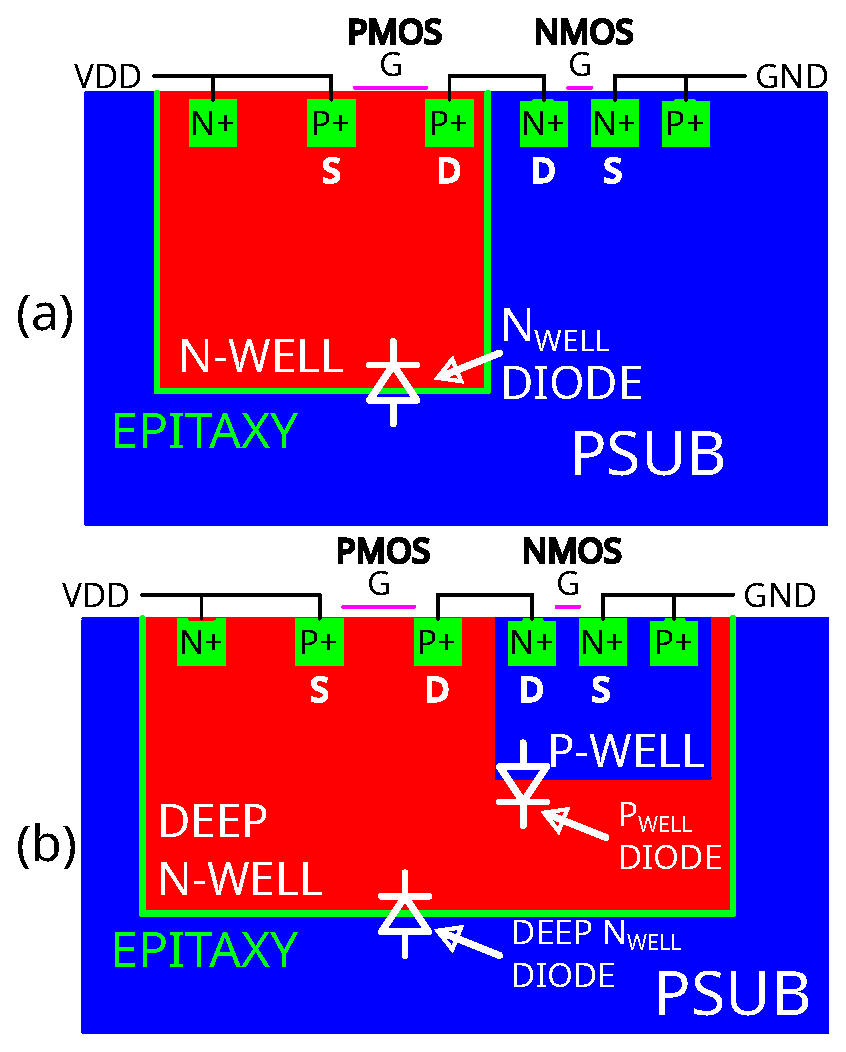
\includegraphics[width=3in]{DUAL+TRIPLE.eps}
\caption{Side view of an inverter in a dual-well (a), and a triple-well (b) silicon substrates.}
\label{fig_dual_triple}
\end{figure}

\subsection{Triple-well standard-cells model}
In \cite{mybbi} was introduced an electrical model allowing to simulate the distribution of BBI pulses through dual-well substrates. In this former work, as it is done in \cite{mathieuEMFI}, the IC surface is split in Standard-Cell Segments (SCS), according to the topology of the power delivery network, as illustrated in Fig. \ref{fig_scs_p}.
Each SCS, which is a rectangle of length $l$ ($30 \; \mu m$ in this paper) and height $h$ ($5 \; \mu m$ in this paper) is a portion of the considered IC, circumscribed at the top level by the power rails (in red and orange) and at the bottom by the substrate junction (the green layer). Depending on $h$ and $l$, a SCS can contain between fifty and two hundreds CMOS logic gates.

\begin{figure}[!t]
\centering
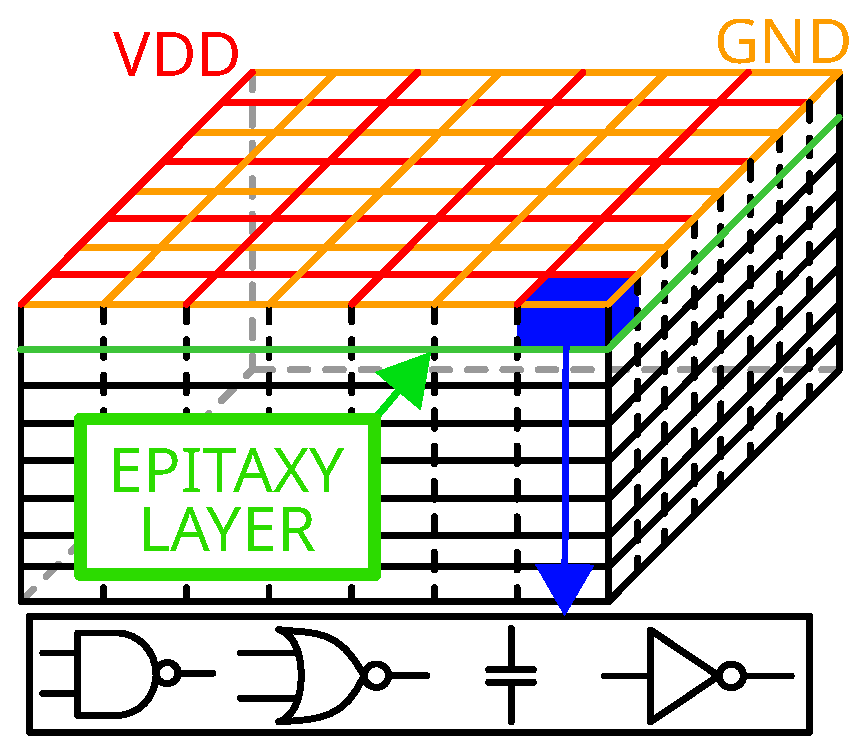
\includegraphics[width=2.5in]{IC_3D_STD_CELL.eps}
\caption{IC surface splitting in Standard Cells Segments}
\label{fig_scs_p}
\end{figure}

\begin{figure}[!t]
\centering
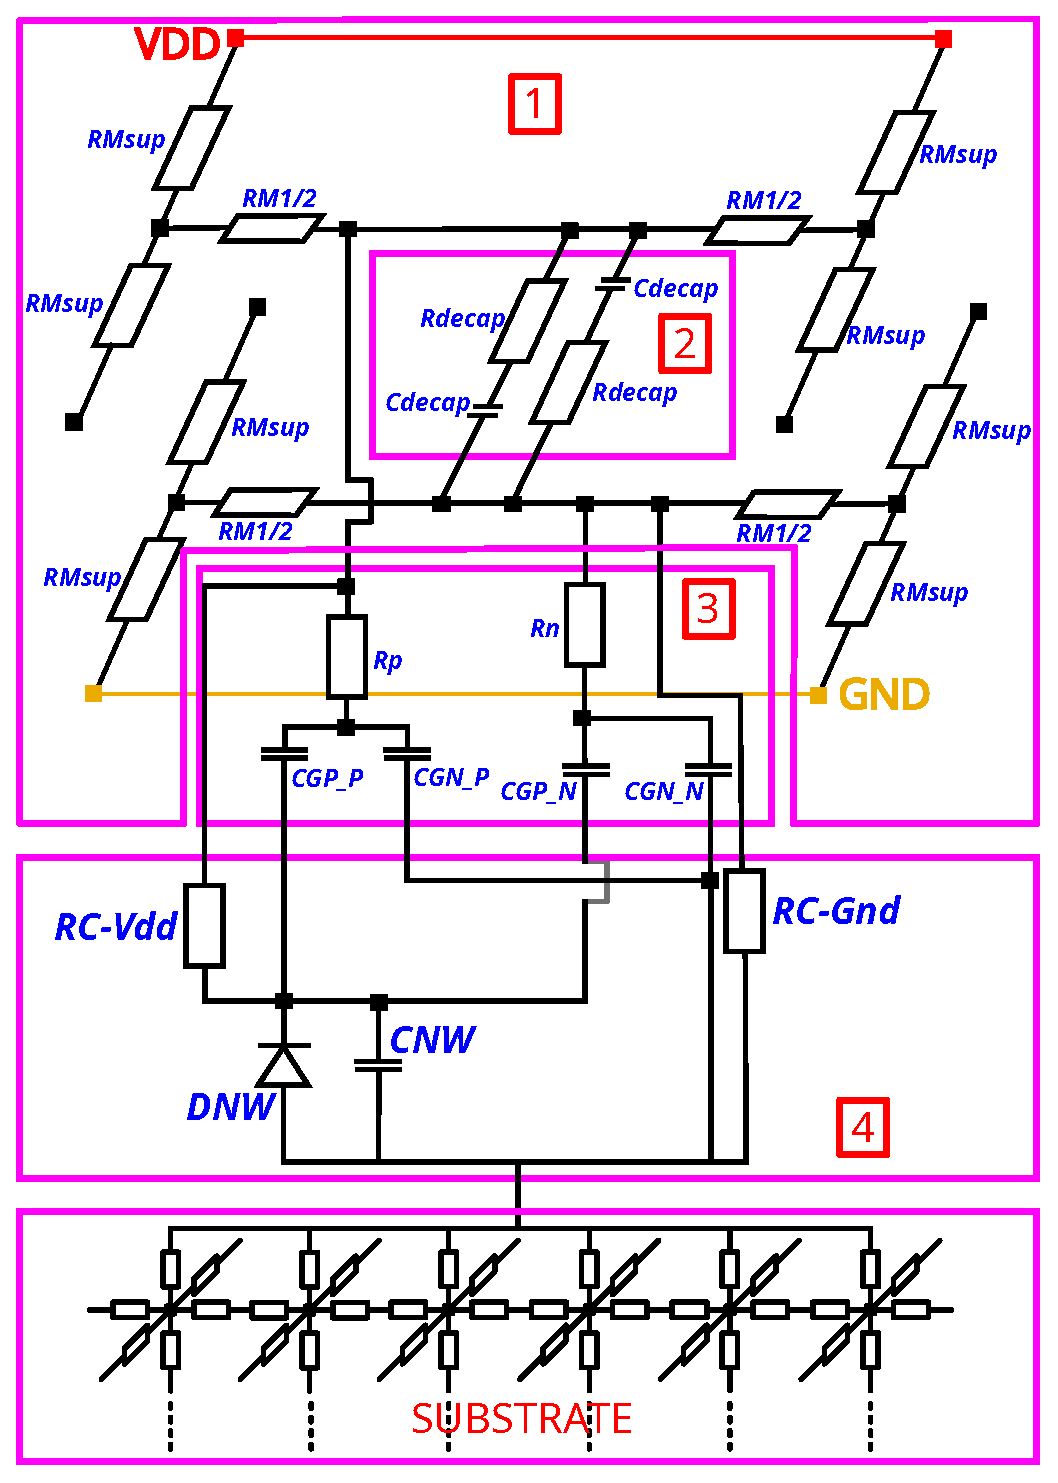
\includegraphics[width=2.5in]{SCS_DW.eps}
\caption{SCS electrical model for dual-well ICs.}
\label{fig_scs_dw}
\end{figure}

Fig. \ref{fig_scs_dw} presents the detailed electrical schematic of a SCS for a dual-well substrate that was used in \cite{mybbi} to study the effects of ICs substrate thinning on BBI efficiency. Region \fbox{1} represents the power rails routing across two metal levels, \fbox{2} the decoupling capacitors that exist between the power rails, \fbox{3} models the standard cell logic gates, \fbox{4} is the $N_{well}$, which is then connected below to the substrate.

Despite its accuracy for dual-well substrates, it cannot be used to simulate the BBI disturbance distribution through triple-well substrates, so it has been improved for this purpose.

The resulting model is given in Fig. \ref{fig_scs_tw} and new areas are colored in green. As before, region \fbox{1} models the power rails routing, \fbox{2} the decoupling between both power rails, \fbox{3} the $Deep N_{well}$ with its PMOS transistors and \fbox{3'} the $P_{well}$ with its NMOS transistors, buried inside the deep $N_{well}$. Then, \fbox{4} reports the deep $Deep N_{well}-P_{well}$ junction. Finally, \fbox{5} describes the $P_{substrate}-Deep N_{well}$ silicon junction, connected to the substrate layer.

\begin{figure}[!t]
\centering
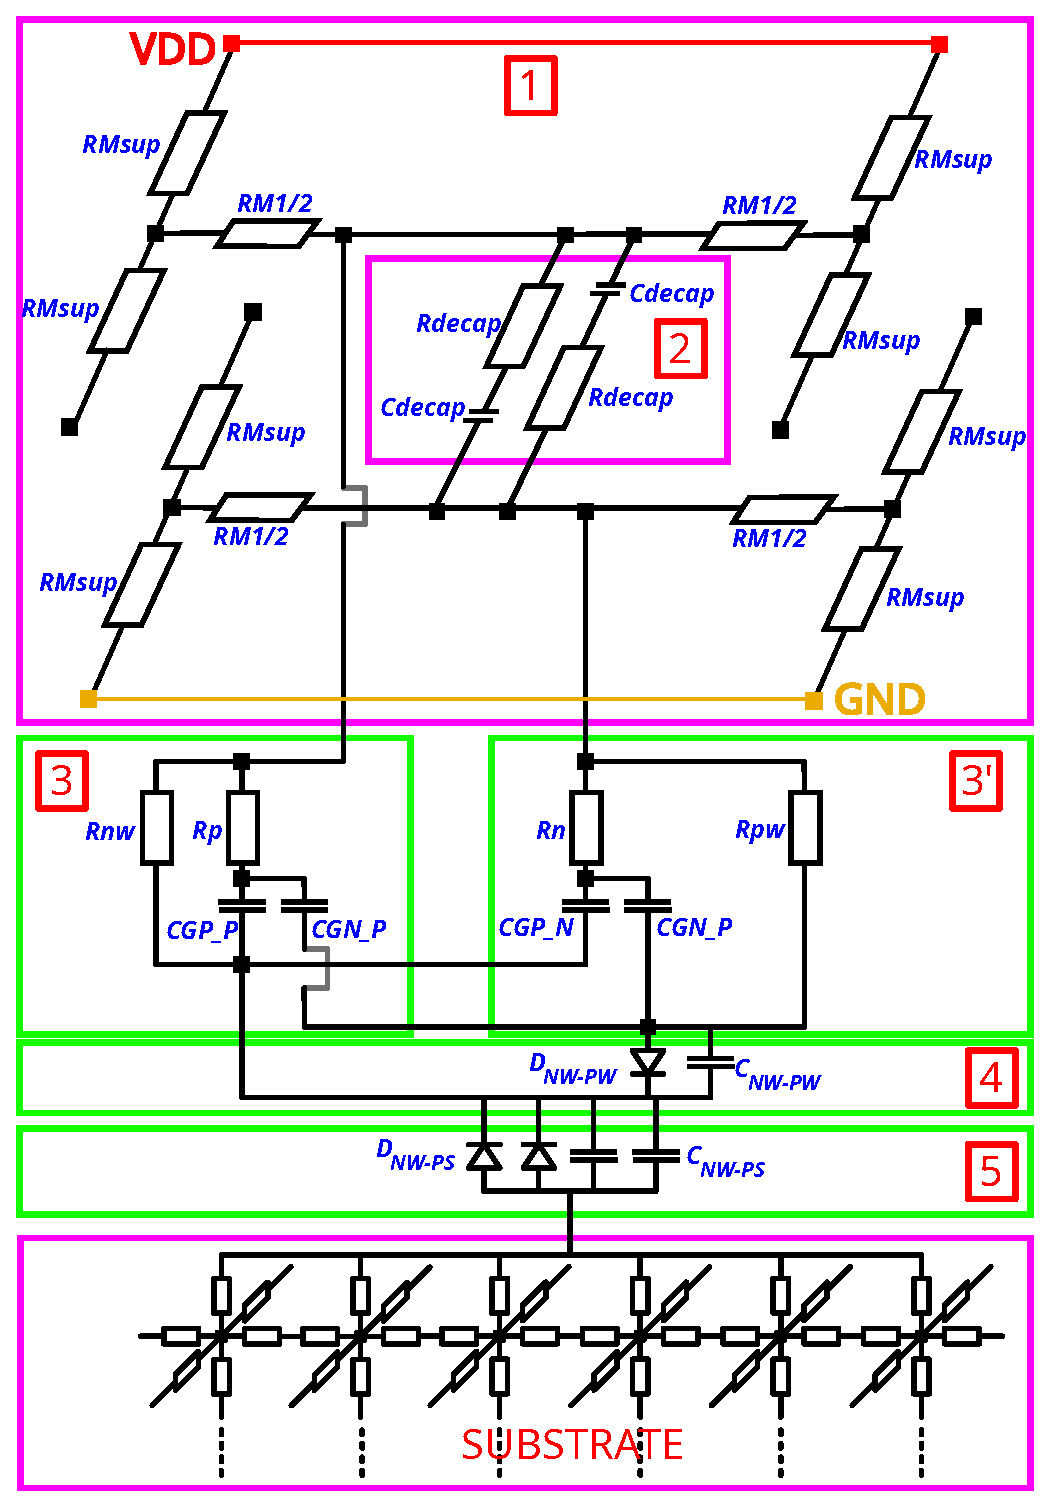
\includegraphics[width=2.5in]{SCS_TW.eps}
\caption{SCS electrical model for triple-well ICs.}
\label{fig_scs_tw}
\end{figure}

\subsection{Simulation methodology}
While one can guess that the electrical coupling between the BBI tip end and the power rails is different in nature for dual-well and triple-well substrates, it remains difficult to finely predict this difference by a simple analysis of both models. It is thus necessary to perform simulations.

Two different IC models were thus developed: one for a dual-well substrate and one for a triple-well substrate. It was achieved with custom Python scripts duplicating and connecting 7000 SCS between them. It allowed to model a matrix of 200 SCS rows and 35 SCS columns. It is equivalent to two ICs with an approximate surface of $1 \; mm ^2$. The substrate thickness, without loss of generality, was chosen to be equal to $140 \; \mu m$. The BBI tip end considered during these simulations measures $30 \; \mu m \times 30 \; \mu m$ and is positioned at the center of the considered IC.

During the simulations, a specific attention was paid to critical currents and voltages inside the ICs in order to disclose what is happening during BBI. Among those were selected:
\begin{itemize}
\item The voltage of the lower level metal rails (Metal 1) of the power and ground grids: $VDD(t)$ and $GND(t)$.
\item The voltage distribution $V_{SUB}(t)$ all over the substrate to analyze potential difference in the distribution of the disturbance through dual-well and triple-well substrates.
\item The voltage of the epitaxy layer $V_{EPI}(t)$, which is the junction between the substrate and the CMOS logic gates.
\end{itemize} 

The computer used to perform these simulations features a 3 GHz 48 cores 96 threads CPU and has 460 GB of available memory. The time required to simulate the behavior of these $1 \; mm \times 1 \; mm \times 140 \; \mu m$ ICs during $60 \; ns$ is about 4 hours for one set of conditions, while the peak memory usage is about $100 \; GB$.

For the sake of readability, only most valuable results are given and their analysis is split in two parts. One for positive pulses and the other one for negative pulses. It is also split in two aspects: time related local simulation results and spatial overall simulation results.

\begin{figure*}[!hbtp]
\centering
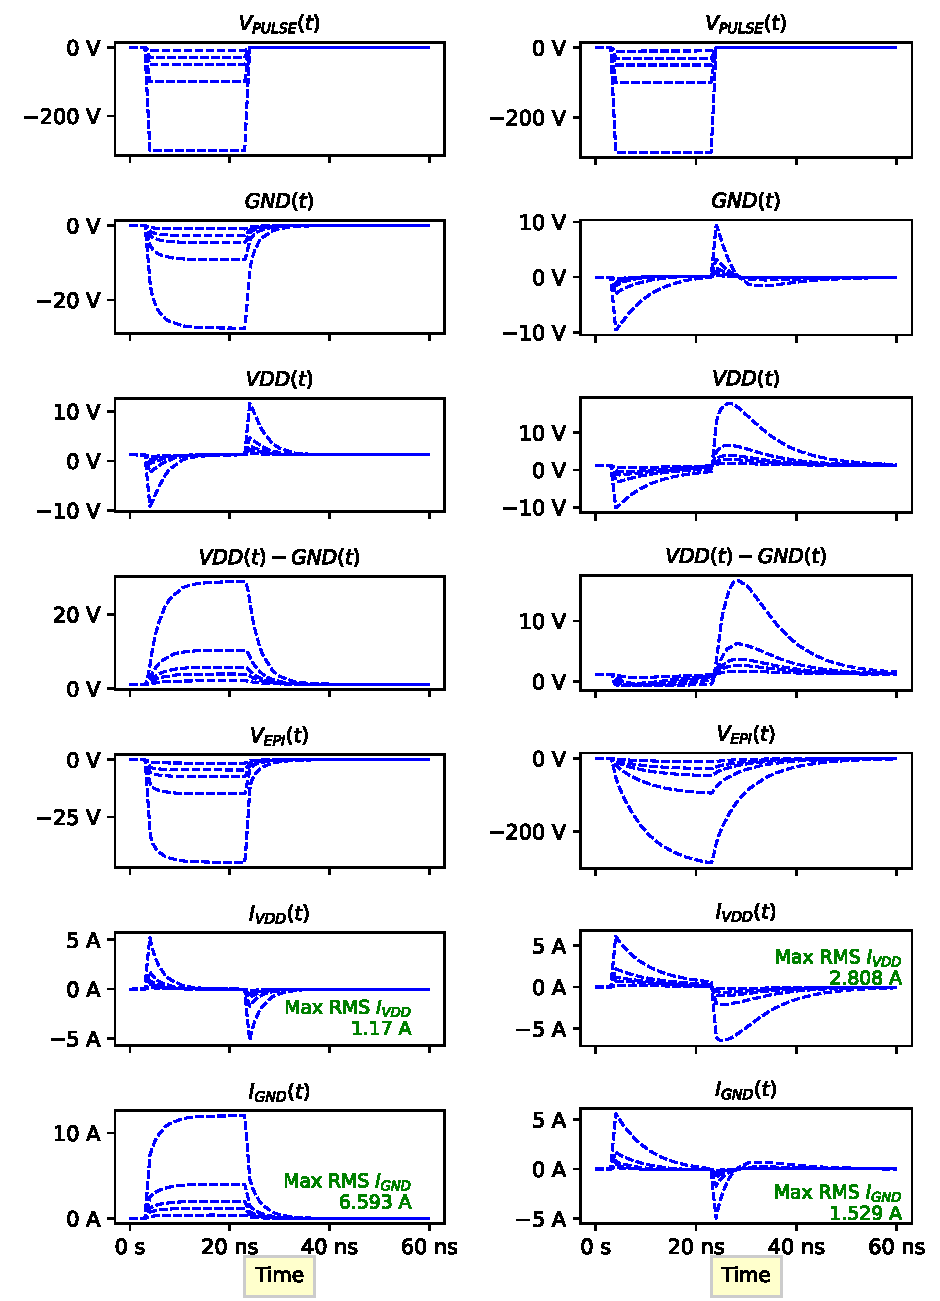
\includegraphics[width=6in]{NEGATIVE_COMP.pdf}
\caption{20ns negative polarity BBI in a dual-well (left) and a triple-well (right) SCS.}
\label{fig_neg_comp}
\end{figure*}

\begin{figure*}[!hbtp]
\centering
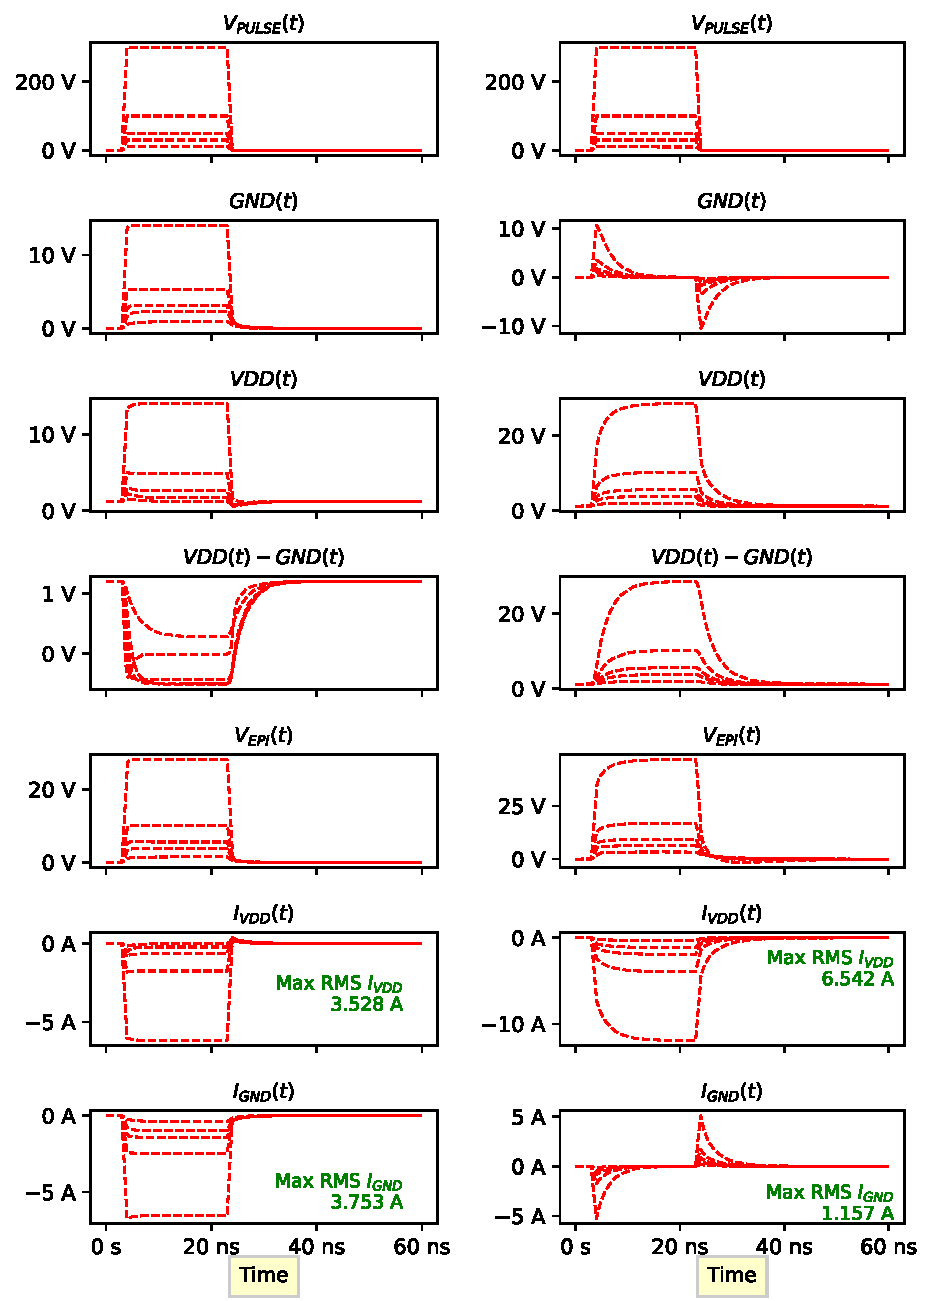
\includegraphics[width=6in]{POSITIVE_COMP.pdf}
\caption{20ns positive polarity BBI in a dual-well (left) and a triple-well (right) SCS.}
\label{fig_pos_comp}
\end{figure*}

\begin{figure}[!ht]
\centering
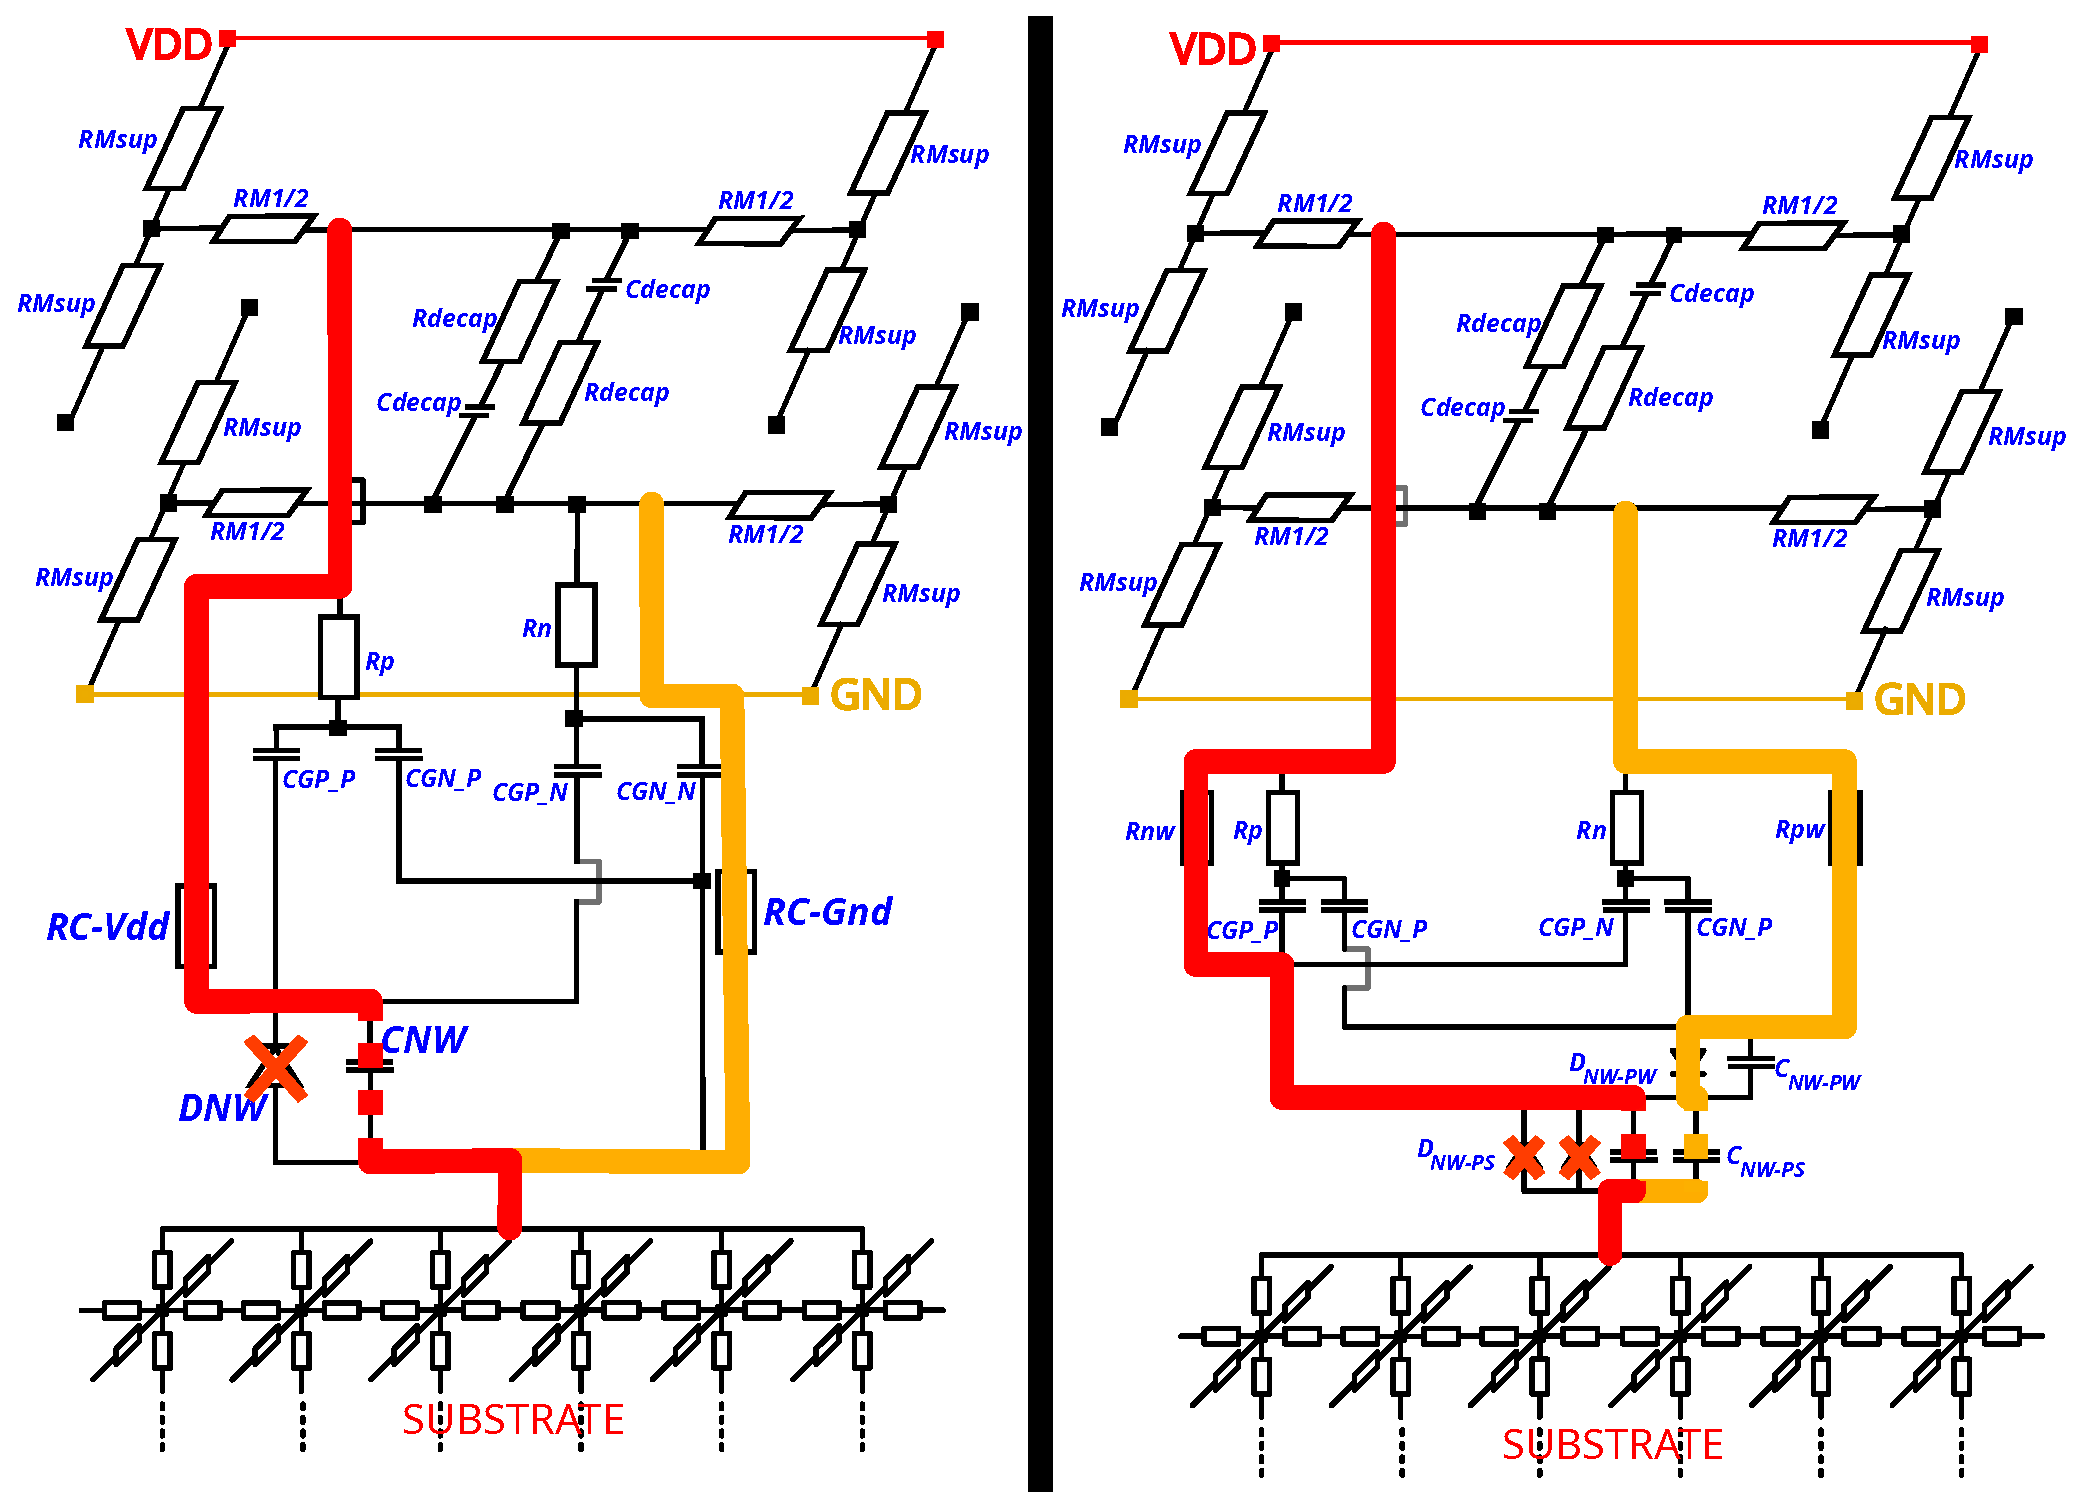
\includegraphics[width=3.3in]{neg_path_comp.eps}
\caption{Electrical paths followed by the negative BBI voltage pulse to flow out of the IC by the GND (yellow) and VDD (red) pads in dual-well (left) an triple-well (right) ICs.}
\label{fig_neg_path}
\end{figure}

\begin{figure}[!ht]
\centering
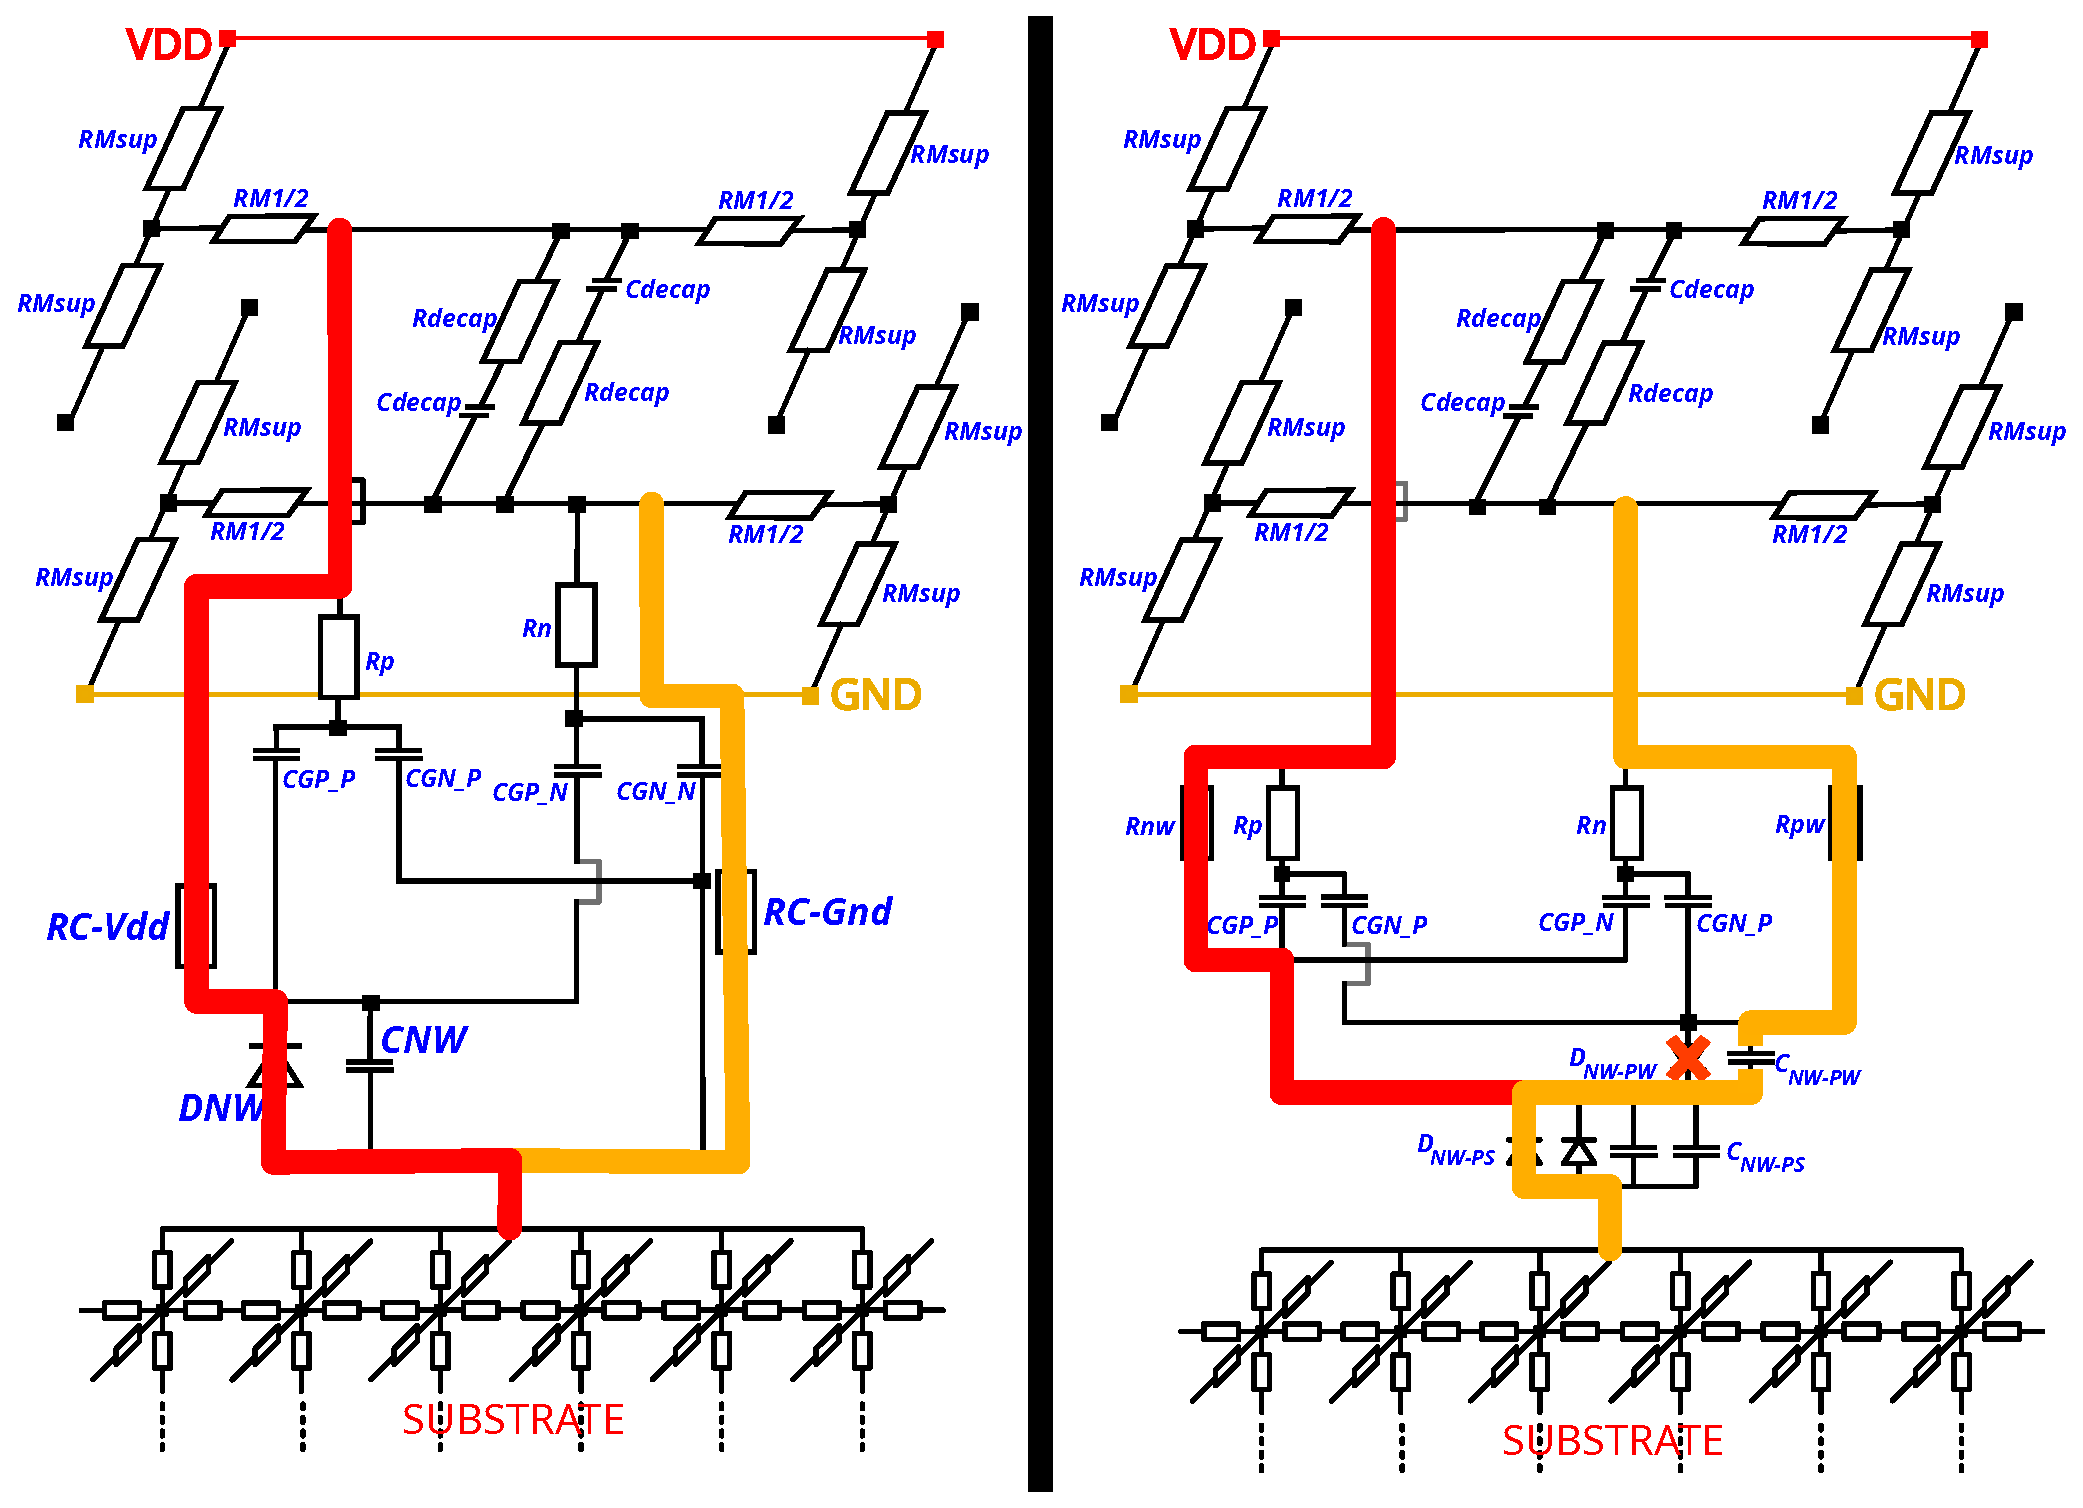
\includegraphics[width=3.3in]{pos_path_comp.eps}
\caption{Electrical paths followed by the positive BBI voltage pulse to flow out of the IC by the GND (yellow) and VDD (red) pads in dual-well (left) an triple-well (right) ICs.}
\label{fig_pos_path}
\end{figure}

\subsection{Time-related local simulation results}
Performing these simulations allowed to evaluate the differences in behavior of the SCS located above the BBI probe concerning dual-well and triple-well substrates.

\subsubsection{Negative pulses}
Fig. \ref{fig_neg_comp} gives the noteworthy voltages and currents during BBI with voltage pulses ranging between $-10 \; V$ and $-300 \; V$.

In the case of a dual-well substrate, the N-well diode is reverse biased (turned off). The coupling between the probe and $VDD$ is only ensured by $C_{NW}$ (see Fig. \ref{fig_neg_comp}) and is therefore capacitive. It can also be observed in Fig. \ref{fig_neg_path} on the left. Indeed, the waveform of $VDD$ looks like two sawtooth peaks with opposite polarities. This is the typical capacitive response to two opposite stimuli. On the contrary, the coupling with $GND$ is resistive. It is once again visible in Fig. \ref{fig_neg_comp}: $GND$ has a waveform similar to the setpoint with a lower response time.

Regarding the triple-well substrate, the $Deep N_{well}$ diode ($D_{NW-PS}$ in Fig. \ref{fig_scs_tw}) is forward biased (turned on) and the $N_{well}$ diode ($D_{NW-PW}$ in Fig. \ref{fig_scs_tw}) is reverse biased, as shown in Fig. \ref{fig_neg_path} on the right. As a result, the coupling between the probe and the supply rails $VDD$ and $GND$ is capacitive, as illustrated by the waveforms in Fig. \ref{fig_neg_comp}.

These different behaviors result in different impacts on the local supply voltage $VDD(t) - GND(t)$ seen by the logic gates. Concerning the dual-well circuit, BBI induces large overshoots on $VDD(t) - GND(t)$. The situation is different regarding the triple-well IC. A BBI induces at first a voltage undershoot set to $-0.6\; V$ by the $P_{well}$ diode. This undershoot lasts for the duration of the pulse, ending with the second edge. After that, $VDD(t) - GND(t)$ experiences a significant overshoot.

\subsubsection{Positive pulses}
Fig. \ref{fig_pos_comp} shows the same results as Fig. \ref{fig_neg_comp} concerning positive BBI pulses, while Fig. \ref{fig_pos_path} shows the charges paths from the substrate to the power rails for positive pulses.

In the case of the dual-well IC, the $P_{well}$ diode is forward biased. There is thus two resistive paths, with different effective resistances between the probe and the supply rails. The coupling is hence resistive and induces a clamping of $VDD(t) - GND(t)$ to $-0.6 \; V$ because of the $N_{well}$ diode. This undershoot lasts until the second edge of the pulse that starts the recovery process of the IC normal bias.

Regarding the triple-well IC, the $Deep N_{well}$ diode is forward biased, while the $P_{well}$ diode is reverse biased. Accordingly, there is a resistive coupling between the tip end and $VDD$, and a capacitive coupling with $GND$. The overall effect is an overshoot of $VDD(t) - GND(t)$ that stands for the duration of the pulse.

\subsubsection{Overview}
Up to this point, only the nature of the electrical couplings between the tip end and both $VDD$ and $GND$ rails has been studied. This analysis provided the results available in Table \ref{table1}.

\begin{table*}[!t]
\centering
% increase table row spacing, adjust to taste
\renewcommand{\arraystretch}{2.5}
\caption{Coupling nature of power grids.}
\label{table1}
\centering
% Some packages, such as MDW tools, offer better commands for making tables
% than the plain LaTeX2e tabular which is used here.
\begin{tabular}{|c||c|c|c|c|}
\hline
& Negative pulses & Positive pulses\\
\hline
Dual-well &
\makecell{Case \textnumero 1\\Capacitive path to $VDD$\\Resistive path to $GND$} &
\makecell{Case \textnumero 2\\Resistive path to $VDD$\\Resistive path to $GND$}\\
\hline
Triple-well &
\makecell{Case \textnumero 3\\Capacitive path to $VDD$\\Capacitive path to $GND$} &
\makecell{Case \textnumero 4\\Resistive path to $VDD$\\Capacitive path to $GND$}\\
\hline
\end{tabular}
\end{table*}

Let us now analyze the effects of BBI in other cases, with respect to the injected current ($I_{INJ}$) in the ICs.

This current necessarily has to flow out of the IC, following both available paths: the path towards $VDD$ rail and the other one towards $GND$ rail. As a result, $I_{INJ} = I_{VDD} + I_{GND}$.

As illustrated in Fig. \ref{fig_neg_comp} and Fig. \ref{fig_pos_comp}, capacitive coupling paths are significantly less efficient to convey current on a given time window compared to resistive paths. Indeed, in the case of a capacitive coupling, charges flow only at the edges of the pulse. Therefore, $I_{INJ}$ flows mostly out of the ICs following resistive paths, if any.

Following this observation, results displayed in Fig. \ref{fig_neg_comp} and \ref{fig_pos_comp} and Table \ref{table1}, one can set up Table \ref{table2}, related to the RMS currents flowing out of the IC. It gives a simplified and more intuitive view of BBI effects.
\begin{table*}[!t]
\centering
% increase table row spacing, adjust to taste
\renewcommand{\arraystretch}{2.5}
\caption{Distribution of the current.}
\label{table2}
\centering
% Some packages, such as MDW tools, offer better commands for making tables
% than the plain LaTeX2e tabular which is used here.
\begin{tabular}{|c||c|c|c|c|}
\hline
& Negative pulses & Positive pulses\\
\hline
Dual-well &
\makecell{$I_{VDD} \approx 0$\\$I_{GND} \approx I_{INJ}$} &
\makecell{$I_{VDD} \approx I_{INJ} \cdot (\frac{1}{2} - \alpha)$\\
          $I_{VDD} \approx I_{INJ} \cdot (\frac{1}{2} + \alpha) $}\\
\hline
Triple-well &
\makecell{$I_{VDD} \approx I_{INJ} \cdot (\frac{1}{2} + \alpha)$\\
          $I_{VDD} \approx I_{INJ} \cdot (\frac{1}{2} - \alpha)$} &
\makecell{$I_{VDD} \approx I_{INJ}$\\$I_{GND} \approx$}\\
\hline
\end{tabular}
\end{table*}
In this Table, $\alpha$ models the impedance differences the paths to $VDD$ and $GND$ rails.

This table can then be translated into Table \ref{table3}, giving the effects of BBI on $VDD(t)$, $GND(t)$ and $VDD(t) - GND(t)$.
\begin{table*}[!t]
\centering
% increase table row spacing, adjust to taste
\renewcommand{\arraystretch}{2.5}
\caption{Effects of BBI on an IC power rails.}
\label{table3}
\centering
% Some packages, such as MDW tools, offer better commands for making tables
% than the plain LaTeX2e tabular which is used here.
\begin{tabular}{|c||c|c|c|c|}
\hline
& Negative pulses & Positive pulses\\
\hline
Dual-well &
\makecell{Negative pulse on $GND$\\Positive pulse on $VDD-GND$} &
\makecell{Positive pulse on $VDD$ and $GND$\\Positive or negative pulse on $VDD-GND$ depending on $\alpha$ value}\\
\hline
Triple-well &
\makecell{Two consecutive sawtooth pulses on both $VDD$ and $GND$\\Clamping and overshoot of $VDD-GND$} &
\makecell{Positive pulse on $VDD$\\Positive pulse on $VDD-GND$}\\
\hline
\end{tabular}
\end{table*}
As reported in Table \ref{table3}, BBI has the following effects:
\begin{itemize}
    \item A positive pulse on the local value of $VDD(t) - GND(t)$ for negative (resp. positive) voltage pulses applied to the substrate of dual-well (resp. triple-well) ICs.
    \item An overshoot of $VDD(t) - GND(t)$, clamped to $-0.6 \; V$ by the $N_{well}$ (resp. $P_{well}$) diode when positive (resp. negative) voltage pulses are applied to the backside of dual-well (resp. triple-well) ICs. Regarding triple-well ICs, this clamping is then followed by an overshoot of $VDD(t) - GND(t)$.
\end{itemize}

At this point, it is important to observe in Fig. \ref{fig_neg_comp} and Fig. \ref{fig_pos_comp} that as soon as a resistive path towards $VDD$ or $GND$ rails (or both) exists, the injected current has a high amplitude for a duration nearly equal to the width of the BBI pulse. These cases are dangerous and can lead to the destruction of the ICs when injection repetition rate and pulse width are high (relative to the considered IC). It explains why performing long BBI experiments in case \textnumero 1, 2 and 4 often results in a destruction of the targeted IC.

\begin{figure}[!ht]
\centering
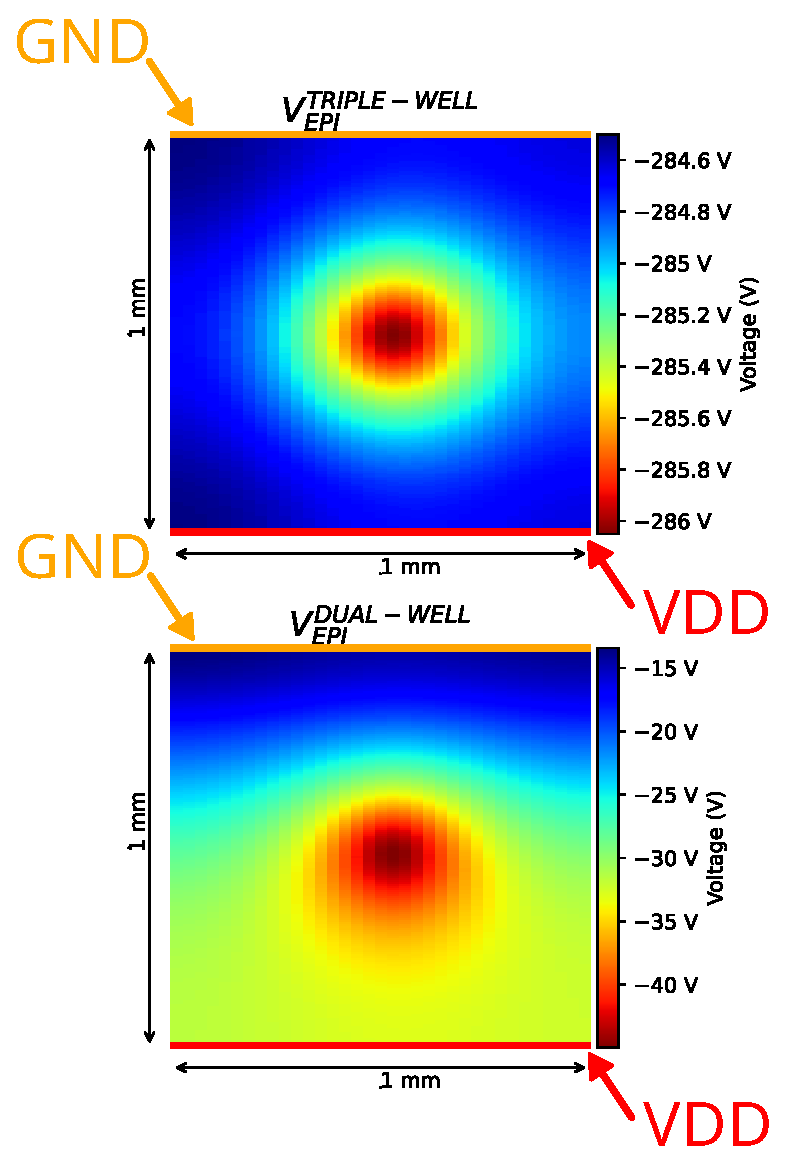
\includegraphics[width=3in]{EPI_VOLT_TR_du.eps}
\caption{Epitaxy voltage distribution at the beginning of the second edge of the pulse (-300V, 20ns) for a triple-well (top) and dual-well (bottom) ICs.}
\label{fig_epi_tw_dw}
\end{figure}
\begin{figure}[!ht]
\centering
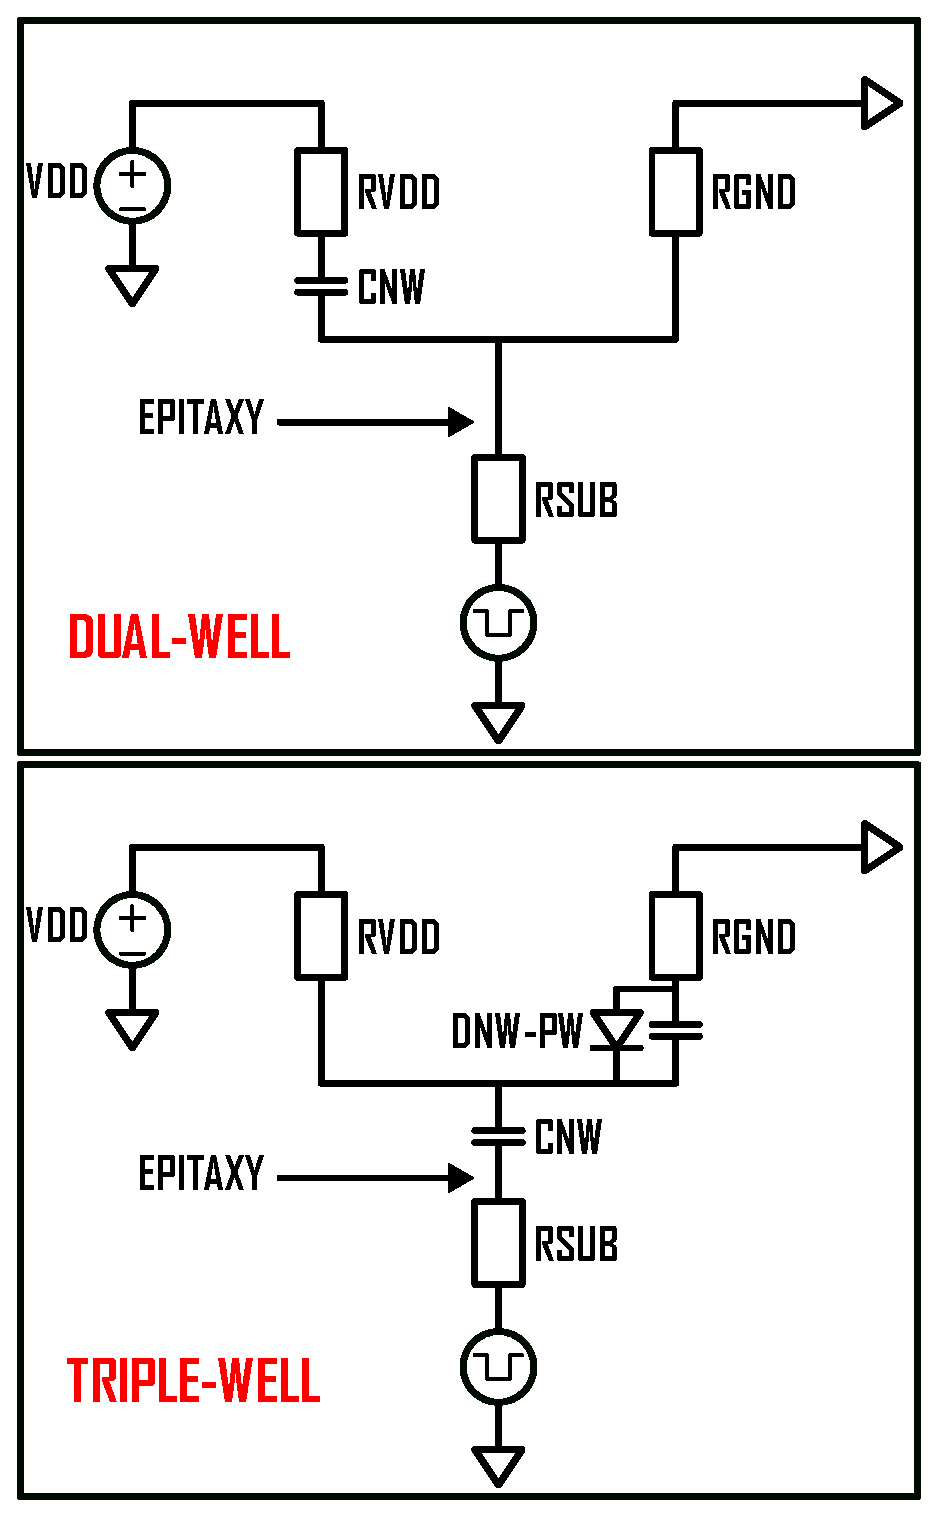
\includegraphics[width=2.5in]{triple-well-grossier-negatif.eps}
\caption{Simplified model of an SCS for a negative pulse.}
\label{fig_epi_gross}
\end{figure}
\subsection{Spatial simulation results}
In the previous section, the BBI effects analysis on dual-well and triple-well ICs focused on the currents and voltages of the SCS located just above the tip end. It was observed that the polarity of the injection, as well as the nature of the substrate have a significant impact on BBI effects.

This section focuses on the spatial distribution of the disturbance at the epitaxy layer (see Fig. \ref{fig_scs_p}) over the entire IC surface.

One can observe that at the end of the BBI impulse plateau, the voltage of the epitaxy layer of triple-well substrates has significantly higher absolute values than the voltage of dual-well substrates ($\simeq285\; V$ vs $\simeq40\; V$). It is explained by the nature of the electrical coupling between the probe (and thus the epitaxy layer) and both $VDD$ and $GND$ rails.

Concerning negative BBI pulses applied to triple-well ICs, the coupling is purely capacitive, while for dual-well ICs it is resistive with $GND$ rail and capacitive with $VDD$ rail. Fig \ref{fig_epi_gross} illustrates the difference between both cases in a simplified way.

As shown, the large signal bias of the epitaxy layer, $V_{EPI}$, of the dual-well IC is explained by the presence of a resistive voltage divider between the substrate and the $GND$ rail, $V_{EPI}$ being:
\begin{equation}
\left|V_{EPI}^{DUAL}\right| = \left|\frac{R_{GND}}{R{GND}+R{SUB}} \cdot V_{PULSE}\right|
\end{equation}
with $R_{SUB}$ being the electrical resistance of the substrate and $R_{GND}$ the resistance between the epitaxy layer and the $GND$ pads. This expression also explains the asymmetry of the dual-well map in Fig. \ref{fig_epi_tw_dw}. Indeed, the closer the $GND$ pad is to the probe location, the lower $R_{GND}$ is, hence the lower voltage.

Regarding the triple-well IC, the resistive couplings between the probe and both $VDD$ and $GND$ rails do not exist. Actually, the couplings are purely capacitive. As a result, $V_{EPI}^{TRIPLE}$ is the voltage present across the capacitor of a $R_{SUB} \cdot C \cdot R_{POWER}$ circuit, $R_{POWER}$ being $R_{VDD} // R_{GND}$. Since $R_{SUB}$ is significantly larger than $R_{POWER}$ (more than 300 times), one can neglect the effect of $R_{POWER}$ and get an approximate expression of the temporal evolution of the epitaxy voltage:
\begin{equation}
\begin{split}
&\left|V_{EPI}^{TRIPLE}\right| \simeq \left|V_{PULSE}\cdot(1-e^{\frac{-t}{R_{SUB} \cdot C_{NW}}})\right|
\\
&V_{EPI}^{TRIPLE} \xrightarrow[t \to +\infty]{} V_{PULSE}
\end{split}
\end{equation}
In addition to this, the absence of any resistive path towards $VDD$ or $GND$ sustains the absence of asymmetry in the top map of Fig. \ref{fig_epi_tw_dw}.

\section{Experimental observations}
\label{section:xp}
Setting up an experiment to verify the soundness of the previously presented models is not an easy task. Indeed, it is quite difficult to monitor the internal voltages of ICs subject to fault injections even using embedded monitors. This major difficulty is furthermore increased by the fact that this work aims at comparing triple-well ICs with dual-well ones.

\subsection{Device under test}
To overcome the above difficulty, an IC featuring both dual-well and triple-well regions on a monolithic die was selected. The considered IC is a modern microcontroller embedding an ARM Cortex M4 core, $2 \; MBytes$ of flash memory and $256 \; kBytes$ of usable RAM. It is designed with a $90 \; nm$ CMOS technology.

Fig. \ref{fig_stm_ir} shows a picture of the device obtained with an infrared camera. On this picture have been overlaid the known triple well region. It corresponds to the placement of the glue logic. Thus, analog blocks and memory arrays are supposedly made out of a dual-well substrate, while no information is available.

\subsection{Experimental setup}
The platform used during these experiments is structured around a voltage pulse generator from AVTECH, the AVRK-4-B-PN. The latter can generate voltage pulses from $\pm 50$ to $\pm 750 \; V$, with a pulse width varying from $6$ to $20 \; ns$. The BBI metal probes are manufactured with a custom 3D-printed housing, to which is attached a spring-loaded metal tip with a diameter of $40 \mu m$, electrically connected to an SMA connector. A Tektronix CT-1 probe has been used to measure the next section currents. It has a typical large bandwidth going from $25 \; kHz$ to $1 \; GHz$. Eventually, a high bandwidth oscilloscope ($1 \; GHz$) was used to acquire the traces required to perform the following experiments. 

\subsection{Experimental protocol}
The experimental validation performed in this paper targeted an observation done in simulations. The latter is related to the difference in amplitude of the electric current flowing out of the IC through the GND pad while performing BBI on dual-well and triple-well ICs. As shown in Fig. \ref{fig_neg_comp}, regarding negative pulses, the current flowing out of the GND pad in a triple-well IC is significantly lower than the one flowing out of the GND pad in a dual-well IC. More precisely, according to the simulations, it comes:
\begin{equation}
max(I_{GND}^{DUAL}) \simeq 2 \cdot max(I_{GND}^{TRIPLE})
\end{equation}

\begin{equation}
RMS(I_{GND}^{DUAL}) \simeq 4.3 \cdot RMS(I_{GND}^{TRIPLE})
\end{equation}
where RMS stands for root mean square.
The purpose of the experiments was to verify whether these relationships are confirmed in practice.

\begin{figure}[!ht]
\centering
\includegraphics[width=3.1in]{STM32_IR_ANN.eps}
\caption{Infrared picture of the microcontroller floorplan under test with triple-well area annotated.}
\label{fig_stm_ir}
\end{figure}

\begin{figure}[!ht]
\centering
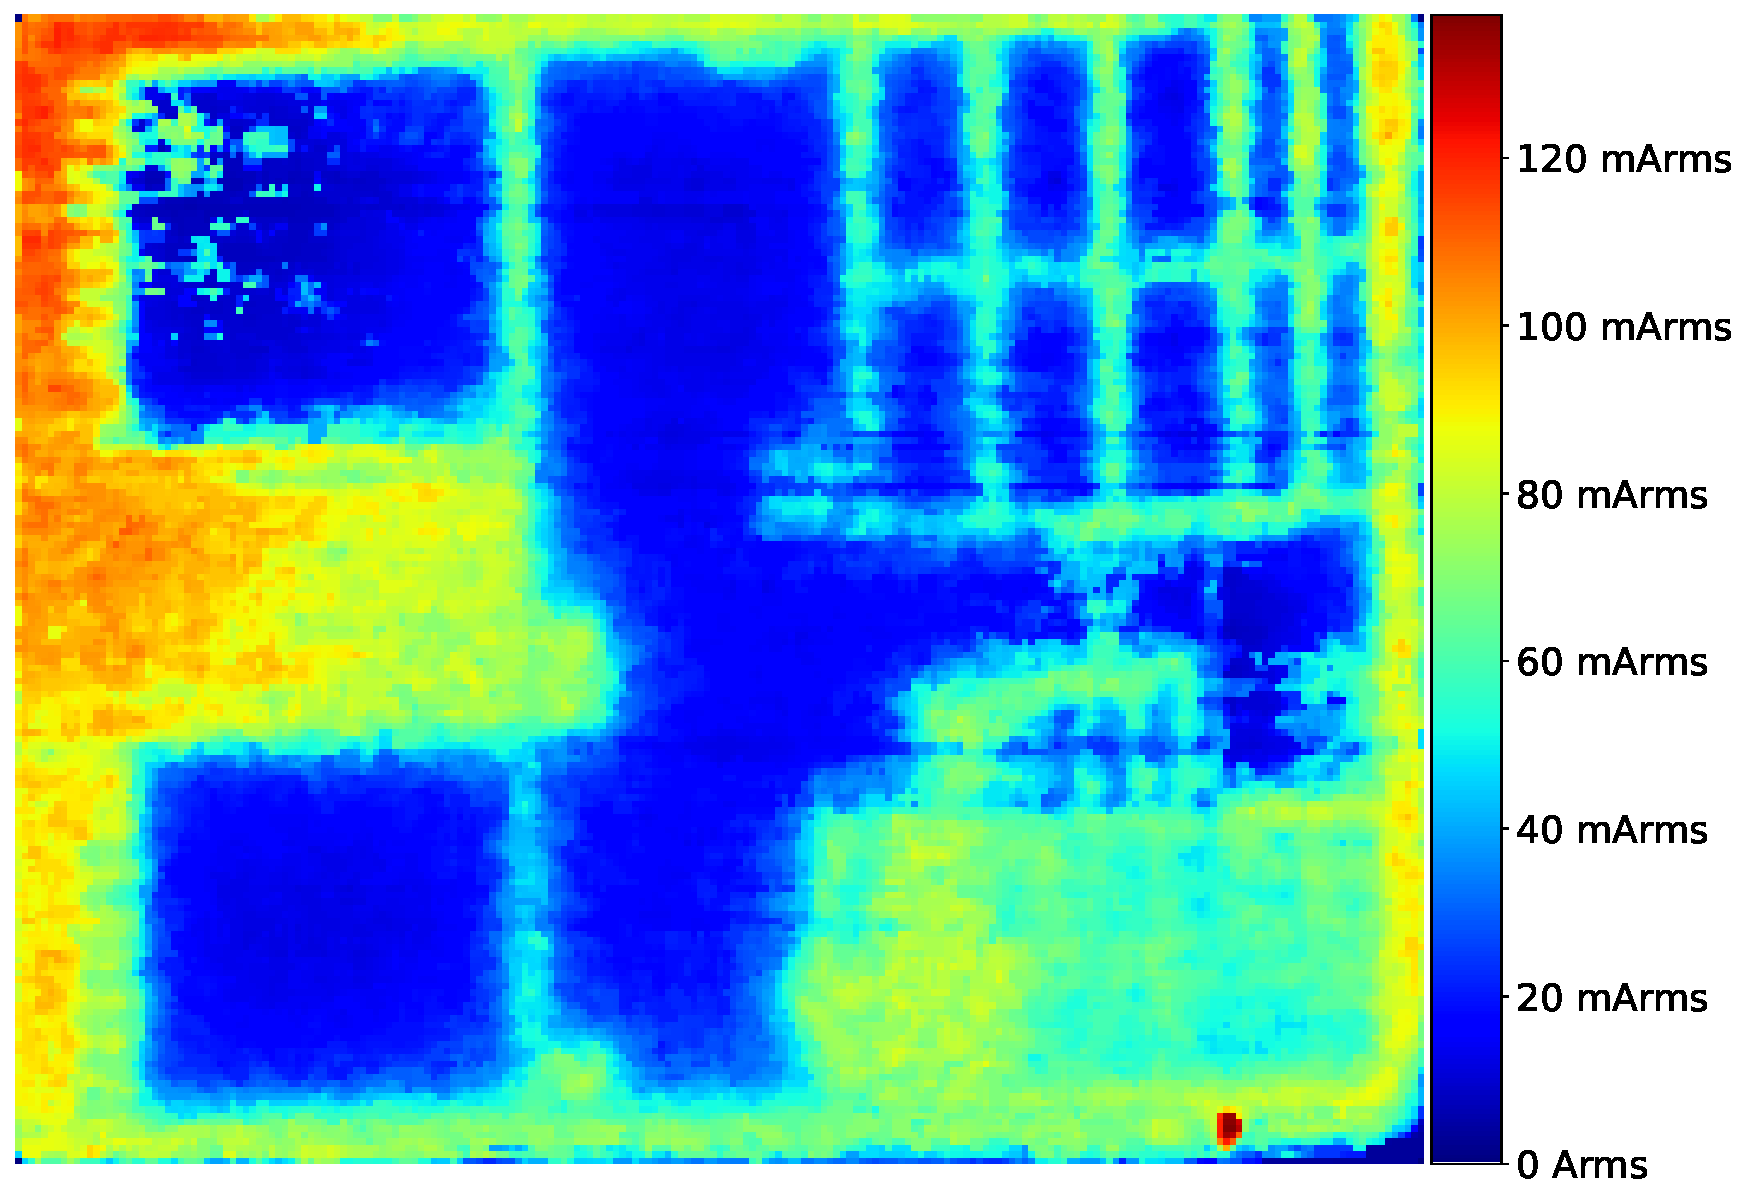
\includegraphics[width=3.1in]{A4_carto11_.pdf}
\caption{Current mapping of a $50 \; \mu m$ thick IC using negative pulses of $70 \; V$ with a PW of $20 \; ns$ with proper grounding.}
\label{fig_carto11}
\end{figure}

\begin{figure}[!ht]
\centering
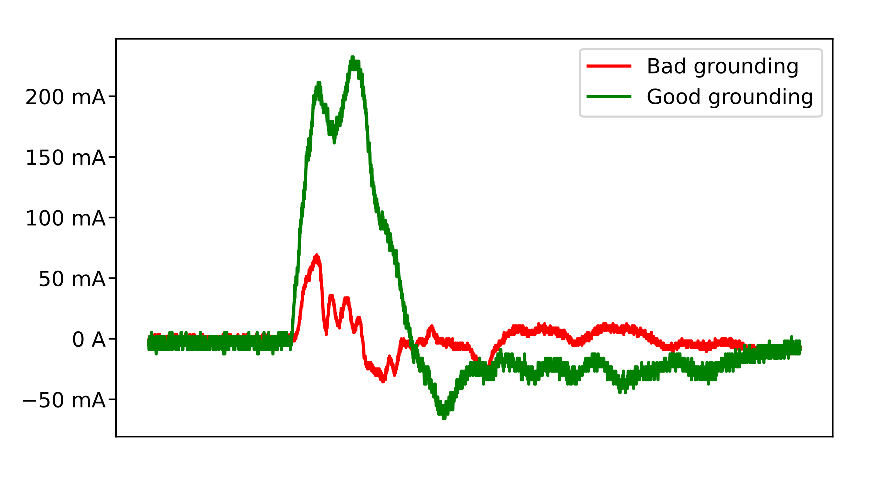
\includegraphics[width=3.1in]{grounding.eps}
\caption{Random traces acquired during the current mapping experiments. Bad grounding (red), better grounding (red).}
\label{fig_traces11}
\end{figure}

\subsection{Experimental measurements}
To compare the simulation results with actual measurements, a scan of the entire IC backside was performed. The displacement step of the tip has been set to $25 \; \mu m$. At each position of the tip, a voltage pulse of amplitude $-70 \; V$ and pulse width equals to $20 \; ns$ was injected. The current flowing through the $GND$ pad was then acquired at each position with the previously described current probe and oscilloscope. From the acquired traces, the RMS values of these currents were computed in order to draw a $I_{GND}^{RMS}$ map.

The resulting map is shown in Fig. \ref{fig_carto11}. Red and blue areas appear. Blue areas correspond to lower RMS current values, red areas to higher RMS current values. As expected, these dark areas enclose the expected and known triple well areas. In addition to this, it seems that the memory arrays of the flash and RAM are also designed over a triple-well substrate area, albeit there is not any confirmation.

Regarding the current ratio, the average value of the RMS current inside the glue logic is between $10\;mA_{RMS}$ and $20\;mA_{RMS}$, while for the analog blocks, it is ranged from $55\;mA_{RMS}$ $65\;mA_{RMS}$. When calculating the experimental ratio of these currents, one can get roughly 4, which is very close to the simulations forecast.
Eventually, as one can observe, this setup can also be used to perform low cost reverse engineering IC imaging instead of infrared pictures to get a rough and inexpensive picture of the IC floorplan.

\begin{figure}[!ht]
\centering
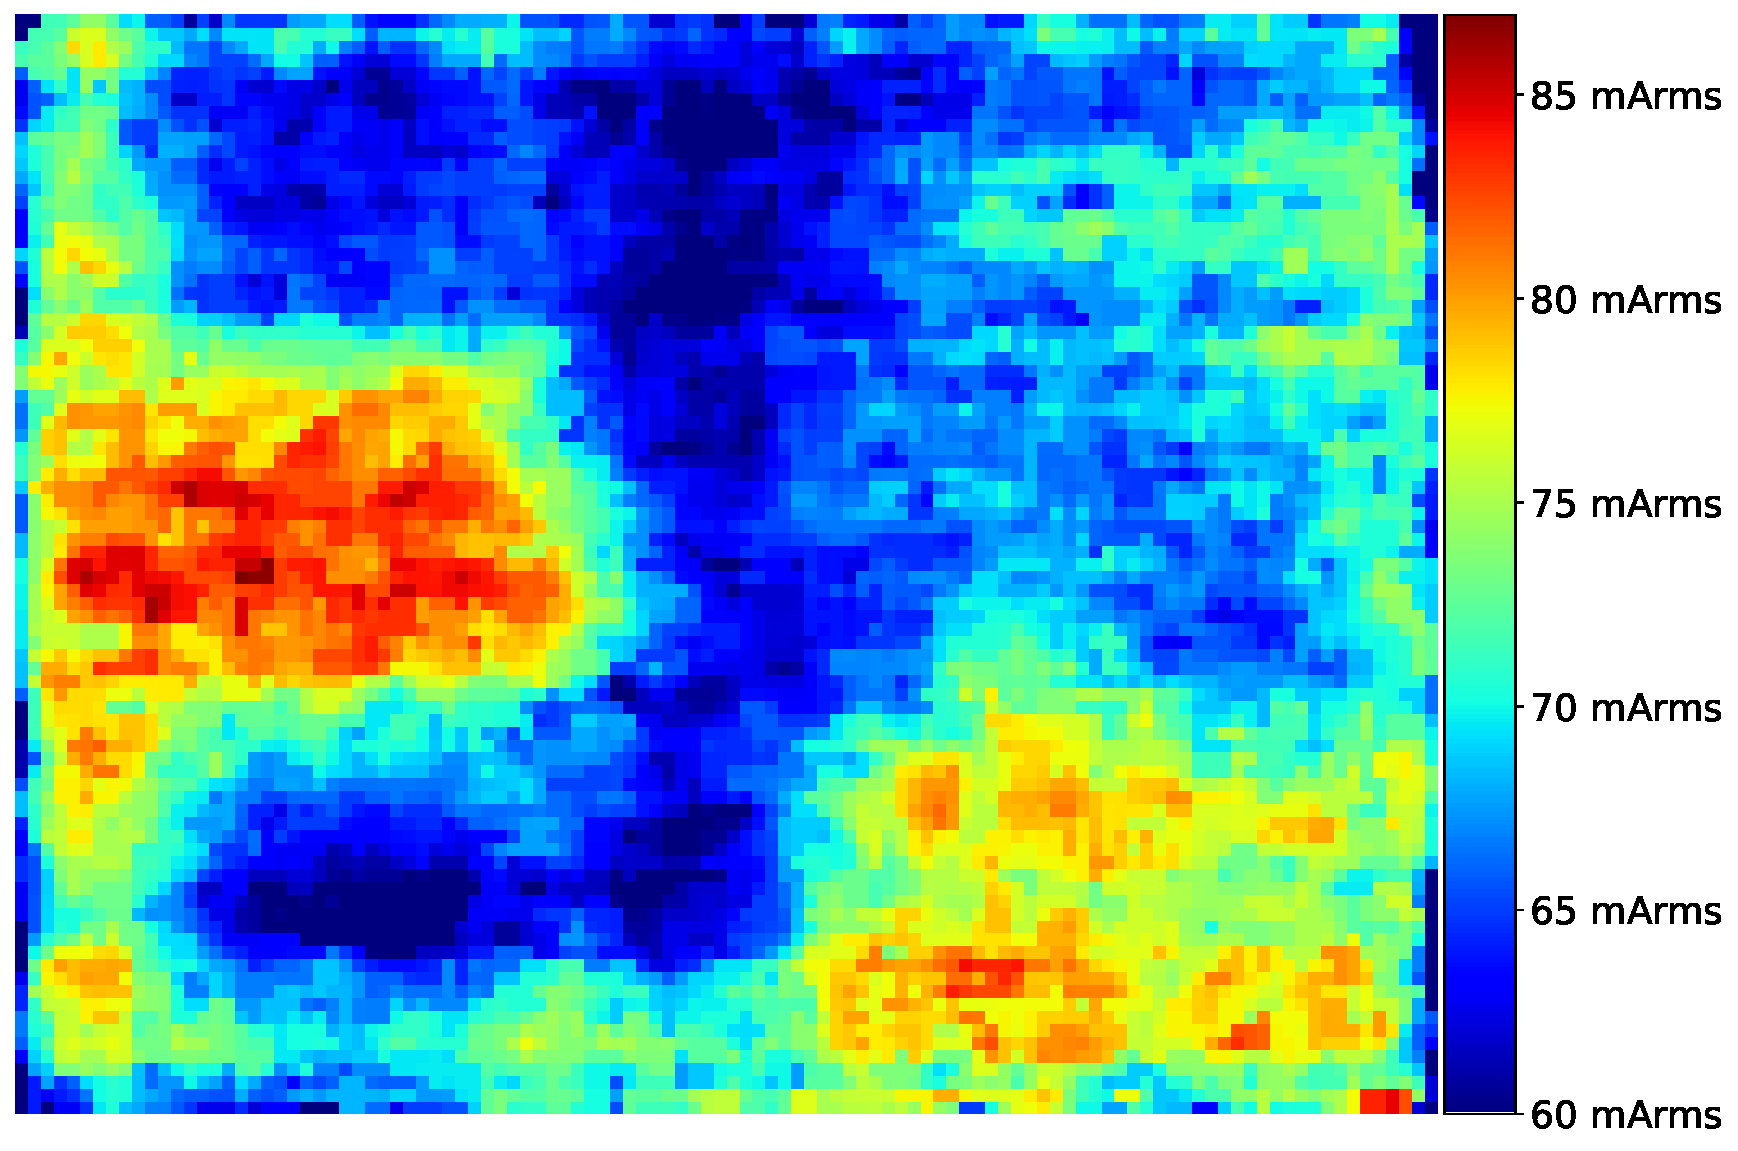
\includegraphics[width=3.1in]{A4_carto3_.pdf}
\caption{Current mapping of a $50 \; \mu m$ thick IC using negative pulses of $70 \; V$ with a PW of $20 \; ns$ with improper grounding.}
\label{carto3}
\end{figure}

\begin{figure}[!ht]
\centering
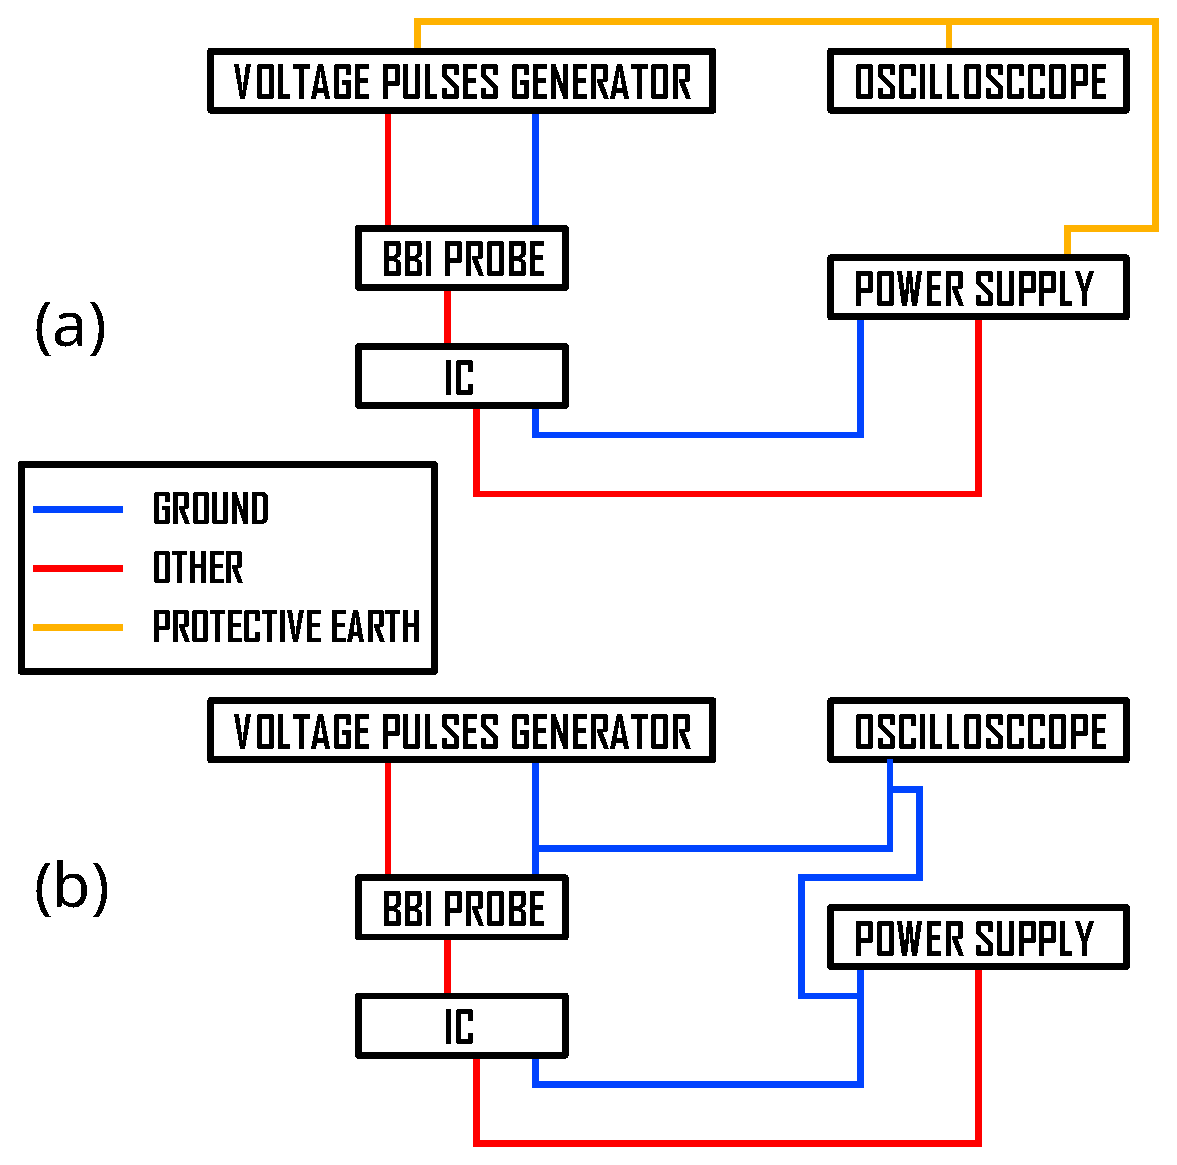
\includegraphics[width=3.1in]{drawing_grounding.eps}
\caption{Schematics of improper (a) and proper (b) groundings between equipment.}
\label{oscillo}
\end{figure}

\subsection{Note about the practice of BBI}
In former works, \cite{pmaurine2012, ktobich2013, nbb2016, oflynn2020, japBBI, mybbi}, BBI was performed by applying the needle to the backside of ICs. Not any information on how to connect the ground of the voltage pulse generator was provided.

According to our observations, it seems that connecting the ground of the voltage generator to a common ground (for instance the ground of the oscilloscope) to the IC and all other equipment provides better results (see Fig. \ref{oscillo}). It avoids letting this bias floating and leads to more powerful (easier fault appearance) and less bouncing injections. Fig \ref{fig_carto11} illustrates these observations. It shows the map of the current flowing out of the IC ground with proper grounding of the voltage generator. This observation is sustained by Fig. \ref{fig_traces11}, where two waveforms of the current flowing out of the IC are shown, acquired on the same spot. The red one was performed with the bad grounding method, the green one through proper equipment grounding. What is notable is the difference in amplitude and in shape: the green one being four times higher and less bouncy. To give an idea of the impact to further highlight the efficiency of this additional wire (the common ground), Fig. \ref{carto3} gives the same map as Fig. \ref{fig_carto11} but realized without proper grounding. The contrast and sharpness of the map are significantly lower. It demonstrates the necessity to properly ground the voltage pulse generator and all the equipment.

\section{Conclusion}
\label{section:concl}
Body biasing injection is an injection technique consisting of applying voltage pulses onto the backside substrate of integrated circuits. As of today, it still has a lot of secrets to reveal. Previous works have demonstrated its efficiency or have studied the effect of substrate thickness on injection properties, but more knowledge is still needed to fully comprehend its behavior. In this context, this work studied the differences in silicon substrates that need to be considered when performing BBI, explaining the differences between dual-well and triple-well substrates with their respective effects on BBI electrical behavior. It was observed that, depending on the polarity of the voltage pulses, the couplings between the metal pin and the power grids differ, thus allowing us to manipulate the IC power grids differently. Finally, a study of BBI effects on dual-well and triple-well substrates was conducted and experiments were performed to verify the accuracy of the study, and some insights were given on how to safely perform BBI.

\begin{thebibliography}{1}
\bibitem{optical}
Skorobogatov, S.P., Anderson, R.J. (2003). Optical Fault Induction Attacks. In: Kaliski, B.S., Koç, ç.K., Paar, C. (eds) Cryptographic Hardware and Embedded Systems - CHES 2002. CHES 2002. Lecture Notes in Computer Science, vol 2523. Springer, Berlin, Heidelberg. https://doi.org/10.1007/3-540-36400-5\_2
\bibitem{pmaurine2012}
Philippe Maurine, Karim Tobich, Thomas Ordas, Pierre yvan Liardet. Yet Another Fault Injection Technique : by Forward Body Biasing Injection. YACC'2012: Yet Another Conference on Cryptography, Sep 2012, Porquerolles Island, France. (lirmm-00762035)
\bibitem{ktobich2013}
K. Tobich, P. Maurine, P. -. Liardet, M. Lisart and T. Ordas, "Voltage Spikes on the Substrate to Obtain Timing Faults," 2013 Euromicro Conference on Digital System Design, 2013, pp. 483-486, doi: 10.1109/DSD.2013.146.
\bibitem{nbb2016}
Noemie Beringuier-Boher, Marc Lacruche, David El-Baze, Jean-Max Dutertre, Jean-Baptiste Rigaud, et al.. Body Biasing Injection Attacks in Practice . CS2: Cryptography and Security in Computing Systems, Jan 2016, Prague, Czech Republic. pp.49-54, (10.1145/2858930.2858940). (lirmm-0143414)
\bibitem{oflynn2020}
Colin O'Flynn.
\newblock Low-cost body biasing injection {(BBI)} attacks on {WLCSP} devices.
\newblock In Pierre{-}Yvan Liardet and Nele Mentens, editors, {\em{CARDIS}
2020, Virtual Event, November 18-19, 2020, Revised Selected Papers}, volume
12609 of {\em Lecture Notes in Computer Science}, pages 166--180. Springer,
2020.
\bibitem{mathieuEMFI}
M. Dumont, M. Lisart and P. Maurine, "Modeling and Simulating Electromagnetic Fault Injection," in IEEE Transactions on Computer-Aided Design of Integrated Circuits and Systems, vol. 40, no. 4, pp. 680-693, April 2021, doi: 10.1109/TCAD.2020.3003287.
\bibitem{lfitriplewell}
Nicolas Borrel, Clément Champeix, Edith Kussener, Wenceslas Rahajandraibe, Mathieu Lisart, et al.. Influence of triple-well technology on laser fault injection and laser sensor efficiency. IEEE International Symposium on Defect and Fault Tolerance in VLSI and Nanotechnology Systems (DFTS 2015), Oct 2015, Amherst, MA, United States. (10.1109/DFT.2015.7315141). (emse-01227366)
\bibitem{techEM}
P. Maurine, "Techniques for EM Fault Injection: Equipments and Experimental Results," 2012 Workshop on Fault Diagnosis and Tolerance in Cryptography, 2012, pp. 3-4, doi: 10.1109/FDTC.2012.21.
\bibitem{phototriple}
Nicolas Borrel, Clément Champeix, Mathieu Lisart, Alexandre Sarafianos, Edith Kussener, et al.. Characterization and simulation of a body biased structure in triple-well technology under pulsed photoelectric laser stimulation. International Symposium for Testing and Failure Analysis (ISTFA), Nov 2014, Houston, United States. (emse-01099035)
\bibitem{mybbi}
Chancel, G., Galliere, JM., Maurine, P. (2022). Body Biasing Injection: To Thin or Not to Thin the Substrate?. In: Balasch, J., O’Flynn, C. (eds) Constructive Side-Channel Analysis and Secure Design. COSADE 2022. Lecture Notes in Computer Science, vol 13211. Springer, Cham. https://doi.org/10.1007/978-3-030-99766-3\_6.
\bibitem{japBBI}
T. Wadatsumi et al., "Voltage Surges by Backside ESD Impacts on IC Chip in Flip Chip Packaging," 2022 IEEE International Reliability Physics Symposium (IRPS), 2022, pp. P14-1-P14-6, doi: 10.1109/IRPS48227.2022.9764457.
\bibitem{chinoisFDSOI}
Cheng K., Khakifirooz A. Fully depleted SOI (FDSOI) technology. Sci. China Inf. Sci. 59, 061402 (2016). https://doi.org/10.1007/s11432-016-5561-5.
\end{thebibliography}
\end{document}
